\section{Wiederholung der Wahrscheinlichkeitsbegriffe}
\begin{merke}{Grundbegriffe der Wahrscheinlichkeit}{}
    Ein Ereignis A ist eine Teilmenge der Ergebnisraumes $\Omega$.\\
    Ein Ereignis A tritt ein, wenn das Versuchsergebnis $\omega$ in A enthalten ist, also wenn gilt: $\omega \in A$.\\
    Alle Elemente von $\Omega$, die nicht zum Ereignis A gehören, fasst man unter dem Namen Gegenereignis $\Bar{A}$ von $A$ zusammen. Damit ist $\Bar{A} = \Omega \setminus A$.
\end{merke}
\begin{b8d}{Mengenalgebra}{}
    \begin{itemize}
        \item Schnittmenge $A\cap B$: Menge der gemeinsamen Ergebnisse von A und B
        \item Vereinigungsmenge $A\cup B$: Menge der Ergebnisse die sowohl in A als auch in B liegen.
    \end{itemize}
\end{b8d}
\begin{merke}{Unvereinbar}{}
Zwei Ereignisse A und B heißen unvereinbar, wenn $A\cap B = \{ \}$.
\end{merke}
\section{Axiomatischer Aufbau der Wahrscheinlichkeit}
Der axiomatische Aufbau der Wahrscheinlichkeitsrechnung geht auf den russischen Mathematiker Kolmogoroff zurück. Hierbei wird versucht, die gesamte Stochastik mit möglichst wenigen Annahmen zu beschreiben. Die sogenannten Axiome sind hierbei Grundannahmen die weder bewiesen noch widerlegt werden können. Hierbei wird die Berechnung der Wahrscheinlichkeit durch eine Funktion $P$ beschrieben.\\
\begin{defi}{}{Grundaxiome der Stochastik}
    Eine Funktion $P$, die jedem Ereignis A eine Wahrscheinlichkeit $P(A)$ zuordnet nennt man Wahrscheinlichkeitsverteilung genau dann wenn sie folgende Eigenschaften erfüllt.
\end{defi}
\section{Bedingte Wahrscheinlichkeit}\index{Wahrscheinlichkeit!bedingte Wahrscheinlichkeit}
Wahrscheinlichkeiten von Ereignissen können sich verändern, wenn bereits andere Ereignisse eingetreten sind. Um diesen Einfluss zu untersuchen, wird der Begriff der bedingten Wahrscheinlichkeit eingeführt.
\begin{defi}{Die bedingte Wahrscheinlichkeit}{}
\index{Bedingte Wahrscheinlichkeit}
   Die Wahrscheinlichkeit eines Ereignisses B unter der Bedingung, dass das Ereignis A bereits eingetreten ist lässt sich durch folgende Zusammenhang berechnen: $$P_A(B) = \dfrac{P(A\cap B)}{P(A)}$$   
\end{defi}
Durch die Betrachtung eines zweistufigen Baumdiagramms ist es möglich, die Definition für die bedingte Wahrsheinlichkeit zu zeigen.
\begin{merke*}{Die Herleitung der bedingten Wahrscheinlichkeit}{}
\begin{multicols}{2}
\scalebox{0.65}{
% allgemeines Layout des Baums
\tikzstyle{level 1}=[level distance=2.5cm, sibling distance=5cm]
\tikzstyle{level 2}=[level distance=2.5cm, sibling distance=4cm]
% definiert Knoten- und Endpunkte
% text width ändert die Boxbreite wobei 1em einem Zeichen entspricht
\tikzstyle{bag} = [circle, draw, text width=1em, inner sep=2pt, text centered]
\tikzstyle{end} = [circle, minimum width=4pt, fill, inner sep=0pt]
\begin{tikzpicture}[grow=down]
  \node[bag]{}
  child
  {
    node[bag] {$A$} % beschriftet Knoten 2 in erster Ebene mit X
    child
    {
      node (B) [bag] {$B$} % beschriftet Knoten 4 in zweiter Ebene mit D
      node [below of = B] {$P(A \cap B)$}
      edge from parent
      node[left]  {$P_{A}(B)$} % beschriftet Verbindung zu Knoten 4 (Ebene 2) mit p
} child {
      node[bag] {$\Bar{B}$} % beschriftet Knoten 3 in zweiter Ebene mit C
      edge from parent
      node[right]  {$P_{A}(\Bar{B})$} % beschriftet Verbindung zu Knoten 3 (Ebene 2) mit m
    }
    edge from parent
    node[left]  {$P(A)$} % beschriftet Verbindung zu Knoten 2 (Ebene 1) mit f
} child {
    node[bag] {$\Bar{A}$} % beschriftet Knoten 1 in erster Ebene mit A
    child
    {
      node[bag] {$B$} % beschriftet Knoten 2 in zweiter Ebene mit B
      edge from parent
      node[left]  {$P_{\Bar{A}}(B)$} % beschriftet Verbindung zu Knoten 2 (Ebene 2) mit k
} child {
      node[bag] {$\Bar{B}$} % beschriftet Knoten 1 in zweiter Ebene mit A
      edge from parent
      node[right]  {$P_{\Bar{A}}(B)$} % beschriftet Verbindung zu Knoten 1 (Ebene 2) mit i
    }
    edge from parent
    node[right]  {$P(A)$} % beschriftet Verbindung zu Knoten 1 (Ebene 1) mit w
  };
\end{tikzpicture}}

Nach der ersten Pfadregel berechnet sich die Wahrscheinlichkeit $P(A\cap B)$ durch das Produkt der einzelnen Pfadwahrscheinlichkeiten. Es gilt damit also $$P(A\cap B) = P(A) \cdot P_{A}(B)$$ und daraus folgt die Beziehung: $$P_{A}(B) = \dfrac{P(A \cap B)}{P(A)}$$
\end{multicols}
\end{merke*}
\begin{bsp}{Beispiel für eine bedingte Wahrscheinlichkeit}{}
Für einen Laplace-Würfel sind folgende Ereignisse gegeben:\\
\begin{enumerate}
    \item Ereignis A: Die geworfenen Augenzahl ist durch drei teilbar.
    \item Ereignis B: Die geworfene Augenzahl liegt zwischen 1 und 4.
\end{enumerate}
Nun soll die Wahrscheinlichkeit von A unter der Bedingung B bestimmt werden.\\
\emph{Es wird also die Wahrscheinlichkeit dafür gesucht, dass die gewürfelte Zahl durch drei teilbar ist unter der Bedingung, dass sie zwischen 1 und 4 liegt.}\\[0.5cm]
Für die Wahrscheinlichkeiten gilt damit folgendes: $$P(A) = \dfrac{2}{6} \hspace{0.2cm} \text{und} \hspace{0.2cm} P(B) = \dfrac{4}{6} $$
\scalebox{0.8}{
% allgemeines Layout des Baums
\tikzstyle{level 1}=[level distance=2.5cm, sibling distance=5cm]
\tikzstyle{level 2}=[level distance=2.5cm, sibling distance=4cm]
% definiert Knoten- und Endpunkte
% text width ändert die Boxbreite wobei 1em einem Zeichen entspricht
\tikzstyle{bag} = [circle, draw, text width=1em, inner sep=2pt, text centered]
\tikzstyle{end} = [circle, minimum width=4pt, fill, inner sep=0pt]
\begin{tikzpicture}[grow=down]
  \node[bag]{}
  child
  {
    node[bag] {$B$} % beschriftet Knoten 2 in erster Ebene mit X
    child
    {
      node (B) [bag] {$A$} % beschriftet Knoten 4 in zweiter Ebene mit D
      node [below of = B] {$P(B \cap A) = \dfrac{1}{6}$}
      edge from parent
      node[left]  {$P_{B}(A)$} % beschriftet Verbindung zu Knoten 4 (Ebene 2) mit p
} child {
      node[bag] {$\Bar{A}$} % beschriftet Knoten 3 in zweiter Ebene mit C
      edge from parent
      node[right]  {$P_{B}(\Bar{A})$} % beschriftet Verbindung zu Knoten 3 (Ebene 2) mit m
    }
    edge from parent
    node[left]  {$P(B)$} % beschriftet Verbindung zu Knoten 2 (Ebene 1) mit f
} child {
    node[bag] {$\Bar{B}$} % beschriftet Knoten 1 in erster Ebene mit A
    child
    {
      node[bag] {$A$} % beschriftet Knoten 2 in zweiter Ebene mit B
      edge from parent
      node[left]  {$P_{\Bar{B}}(A)$} % beschriftet Verbindung zu Knoten 2 (Ebene 2) mit k
} child {
      node[bag] {$\Bar{A}$} % beschriftet Knoten 1 in zweiter Ebene mit A
      edge from parent
      node[right]  {$P_{\Bar{B}}(A)$} % beschriftet Verbindung zu Knoten 1 (Ebene 2) mit i
    }
    edge from parent
    node[right]  {$P(\Bar{B})$} % beschriftet Verbindung zu Knoten 1 (Ebene 1) mit w
  };
\end{tikzpicture}}\\
Die Wahrscheinlichkeit für das Ereignis $A\cap B$ entspricht demjenigen Ereignis, dass sowohl B als auch A eintritt. Das entspricht der Menge die nur aus der Augenzahl 3 besteht und damit der Wahrscheinlichkeit $P(A\cap B) = \dfrac{1}{6}$. Aus dem Baumdiagramm folgt damit: $$P(A\cap B) = P(B) \cdot P_{B}(A)$$ und dadurch $$P_{B}(A) = \dfrac{P(A\cap B)}{P(B)} = \dfrac{\dfrac{1}{6}}{\dfrac{4}{6}}= \dfrac{1}{6} \cdot \dfrac{6}{4} = \dfrac{1}{4} $$.
\end{bsp}
\section{Zufallsgrößen und deren Wahrscheinlichkeiten}
\begin{defi}{Zufallsgrößen und Wahrscheinlichkeitsverteilung}{}\index{Zufallsgröße!Definition}
Eine Funktion $X$, die jedem Ergebnis $\omega$ eines Ergebnisraumes $\Omega$ eine reelle Zahl $x$ zuordnet, heißt \textcolor{red}{Zufallsgröße\footnote{Zufallsgröße $\longrightarrow$ ZG}} X.\\
Jeder Wert $x$ einer ZG $X$ tritt mit einer bestimmten Wahrscheinlichkeit $P(X=x)$ auf. Die Funktion, die jedem Wert $x$ einer ZG $X$ die Wahrscheinlichkeit $P(X=x)$ zuordnet, heißt \textcolor{red}{Wahrscheinlichkeitsverteilung} der ZG $X$.\\

Als Beispiel ist hier $P(X=4) = 0,2$ dargestellt.\\
\begin{center}

\begin{tikzpicture}[>=Stealth, scale=0.8]

% Ergebnisraum Omega (kompakter)
\draw[orange] (0,4.5) ellipse (3.2cm and 0.8cm);
\node[orange] at (3.6,5.3) {Ergebnisraum $\Omega$};
\foreach \i/\x/\y in {
  \omega_1/-2.5/4.7,
  \omega_2/-1.5/4.3,
  \omega_3/-0.5/4.8,
  \omega_4/ 0.5/4.3,
  \omega_5/ 1.5/4.7,
  \omega_6/ 2.5/4.3
}{
  \node at (\x,\y) {\(\i\)};
}

% Wertemenge W
% Blauer Hintergrund unter Achse von 1.5 bis 12
\fill[blue!20] (-1.5,2.9) rectangle (4.5,3.1);
\draw[->] (-2.2,3) -- (5,3) node[right] {$x$};
\foreach \x in {-2,-1,0,1,2,3,4}
  \draw (\x,2.9) -- (\x,3.1) node[below=2pt] {\small \x};
\node[blue] at (4.8,3.4) {Wertemenge $W$};

% Grüner Pfeil: Zufallsgröße X
\draw[->, thick, green!60!black] (0.5,4.2) to[bend left=30] (4,3.1);
\node[green!50!black] at (1.5,3.4) {Zufallsgröße $X$};

% P(X = x)-Achse
\draw[->] (-0.1,1.5) -- (3.6,1.5) node[anchor=west] {$P(X = x)$};

% Tick-Marken und Beschriftungen
\foreach \i/\label in {0/0, 1/0.2,  3/0.6, 5/1} {
  \draw (\i*0.6 + 0.3,1.5) -- ++(0,-0.1); % Markierung
  \node at (\i*0.6 + 0.3,1.2) {\label};   % Beschriftung
}

% Roter Pfeil: zweifach gebogen und zeigt exakt auf 0.2 (bei x=0.9, y=1.5)
\draw[->, thick, red]
  (4,2.9) .. controls (5.2,2.3) and (1.4,1.9) .. (0.9,1.5);

\node[red] at (3.4,2.3) {Wahrscheinlichkeitsverteilung};
\end{tikzpicture}  
    
\end{center}
\end{defi}
\begin{merke}{Kumulative Verteilung}{}\index{Zufallsgröße!Kumulative Verteilung}
Die Funktion F, die bei gegebener Zufallsgröße \(X\) jeder reellen Zahl \(x\) die Wahrscheinlichkeit \(P(X\leq x)\) zuordnet, heißt kumulative Verteilungsfunktion der Zufallsgröße \(X\). Hierfür schreibt man \(F:x \mapsto P(X\leq x)\) mit \(x \in \mathds{R}\) und \(P(X\leq x) \in [0;1]\)
\end{merke}
\begin{b8d}{Eigenschaften der kumulativen Verteilung}{}\index{Zufallsgröße!Kumulative Verteilung!Eigenschaften}
Für eine kumulative Verteilungsfunktion \(F\) gilt:
\begin{itemize}
    \item \(\lim\limits_{x\longrightarrow -\infty} F(x) = 0\) und \(\lim\limits_{x\longrightarrow \infty} F(x) = 1\)\textbf{}
    \item Die Funktion \(F\) ist monoton steigend in \(\mathds{R}\)
    \item Der Graph von \(F\) springt bei \(x\), wenn \(P(X\leq x) \neq 0\) ist. Die Höhe des Sprungs beträgt \(P(X=x)\)
    \item Die Wahrscheinlichkeit \(P(a<X\leq b)\), dass die Zufallsgröße \(X\) einen Wert \(x\) aus dem Intervall \(a<X\leq b\) annimmt, kann als Differenz \(F(b) - F(a)\) berechnet werden.
\end{itemize}
\end{b8d}
\section{Erwartungswert und Varianz}
\begin{defi}{Der Erwartungswert}{}\index{Zufallsgröße!Erwartungswert}
Eine ZG nimmt die Werte $x_1, x_2,\ldots , x_n$ mit den Wahrscheinlichkeiten $P(X=x_1), P(X=x_2), \ldots, P(X=x_n)$ an.\\  Dann heißt der zu erwartende Mittelwert \[\mu =E(X) = \sum\limits_{i=1}^n x_i\cdot P(X=x_i)= x_1\cdot P(X=x_1) + x_2\cdot P(X=x_2) +\ldots + x_n \cdot P(X=x_n)\]
    \textcolor{red}{Erwartungswert} von $X$. 
    \end{defi}
    \begin{bem}{Eigenschaften des Erwartungswertes}{}
        \begin{itemize}
            \item Der Erwartungswert $\mu$ ist häufig \textcolor{red}{kein} Wert, den die ZG annimmt.
            \item Ein Spiel heißt \textcolor{red}{\textbf{fair}}, wenn der Erwartungswert des Gewinns eines Glückspiels für jeden Spieler \(0\) ist.
        \end{itemize}
    \end{bem}
    \begin{defi}{Die Varianz}{}\index{Zufallsgröße!Varianz}
  Eine ZG mit $E(X) = \mu$ nehme die Werte $x_1, x_2,\ldots , x_n$ mit den Wahrscheinlichkeiten $P(X=x_1), P(X=x_2), \ldots, P(X=x_n)$ an. \\ 
  Dann heißt die mittlere quadratische Abweichung von $\mu$ \textcolor{red}{Varianz} von $X$: \[Var(X) = \sum\limits_{i=1}^n \left(x_i - \mu\right)^2 \cdot P(X = x_i)= \left(x_1 - \mu\right)^2 \cdot P(X = x_1) + \ldots + \left(x_n - \mu\right)^2 \cdot P(X = x_n)\]
    \end{defi}
    \begin{bem}{Eigenschaften der Varianz}{}\index{Zufallsgröße!Varianz!Eigenschaften}
       Die Werte einer ZG sind häufig Maßzahlen einer Größe. Folglich ist die Varianz von \(X\) die Maßzahl einer Größe, die im Quadrat gemessen wird. Da dies in der Praxis nicht sehr anschaulich ist, wird mit der Standardabweichung ein neues Maß eingeführt.  
    \end{bem}
    \begin{defi}{Die Standardabweichung}{}\index{Zufallsgröße!Standardabweichung}
Die Standardabweichung $\sigma$ einer ZG $X$ bestimmt sich durch $\sigma = \sqrt{Var(X)}$
    \end{defi}
    \section{Kombinatorik}\index{Kombinatorik}
\begin{enumerate}
    \item Permutation als  Anordnung von $n$ Objekten in einer bestimmten Reihenfolge $\longrightarrow n! = n\cdot ( n-1) \cdot (n-2)\cdot \ldots \cdot 3\cdot  2\cdot 1$
    \item Unterscheidungsmöglichkeiten in einem Urnenexperimentes: Man zieht aus einer Menge mit $n$ Elementen $k-$Elemente heraus\\
    \begin{center}
   \begin{tabular}{|c||c|c|}
    \hline
         &  Mit Reihenfolge & Ohne Reihenfolge\\
           \hline\hline
     Mit Zurücklegen   & $n^k$ & $\binom{n+k-1}{k}$\\
     \hline
     Ohne Zurücklegen & $\frac{n!}{\left(n-k\right)!}$& $\binom{n}{k} = \frac{n!}{k!\left(n-k\right)!}$\\
     \hline
    \end{tabular} 
         
    \end{center}
\end{enumerate}
\begin{merke}{Merksatz zum Binomialkoeffizienten}{}\index{Binomialkoeffizient}
Der Binomialkoeffizient \(\binom{n}{k}\) zählt, wie viele Möglichkeiten es gibt, aus \(n\) verschiedenen Elementen genau \(k\) ohne Reihenfolge auszuwählen:
\[\binom{n}{k}=\frac{n!}{k!(n-k)!}\quad (0\le k\le n).\]
\end{merke}
\begin{b8d}{Der Binomialkoeffizient}{}\index{Binomialkoeffizient}
Eigenschaften des Binomialkoeffizienten
\begin{enumerate}
    \item Der Binomialkoeffizient ist symmetrisch $\longrightarrow \binom{n}{k} = \binom{n}{n-k}$
    \item Besondere Werte des Binomialkoeffizienten $\binom{n}{0}= 1; \binom{n}{1} = n$ und $\binom{n}{n}=1$
\end{enumerate}  
\end{b8d}
\section{Hypergeometrische Verteilung}
\begin{bem}{Urnenmodell und „Ziehen mit einem Griff“}{}\index{Urnenmodell}
Viele Zufallssituationen lassen sich als Urnenmodell beschreiben: Es gibt zwei Arten von Objekten (z.,B. „schwarz/weiß“) und man zieht mehrere auf einmal, also \emph{ohne Zurücklegen}. Dann ist nicht die Reihenfolge entscheidend, sondern nur, \emph{wie viele} Objekte einer Art im Ergebnis liegen. Genau hier taucht der Binomialkoeffizient als Zählwerkzeug auf. Das Standardmodell dahinter heißt \emph{hypergeometrische Verteilung}.\index{Hypergeometrische Verteilung}
\end{bem}
\begin{defi}{Hypergeometrische Wahrscheinlichkeit}{}\index{Hypergeometrische Verteilung!Wahrscheinlichkeitsverteilung}
In einer Urne liegen S „Erfolgskugeln“ (z.,B. schwarz) und N-S „Nichterfolgskugeln“ (z.,B. weiß). Es werden n Kugeln ohne Zurücklegen gezogen.
Für \(k\in\{0,1,\dots,n\}\) heißt
\[P(X=k)=\frac{\binom{S}{k}\binom{N-S}{n-k}}{\binom{N}{n}}\]
die \emph{hypergeometrische Wahrscheinlichkeit}, wobei die ZG \(X\) die Anzahl der gezogenen Erfolgskugeln ist.
\end{defi}
\begin{bsp}{Sechs schwarze, vier weiße Kugeln; fünf auf einmal ziehen}{}
In einer Urne liegen 6 schwarze und 4 weiße Kugeln, insgesamt also \(N=10\). Es werden \(n=5\) Kugeln ohne Zurücklegen gezogen. Gesucht ist die Wahrscheinlichkeit dafür, dass \emph{genau drei} schwarze Kugeln darunter sind \((k=3)\).
\end{bsp}
\begin{rechnung}{Berechnung mit Binomialkoeffizienten}{}
Alle 5-Auswahlen aus 10 Kugeln sind gleich wahrscheinlich:\begin{itemize}
    \item \(\binom{10}{5} \longrightarrow\) Anzahl der Möglichkeiten aus 10 Kugeln 5 auszuwählen 
   \item  Anzahl an Möglichkeiten  3 der 6 schwarzen auszuwählen \(\longrightarrow \binom{6}{3}\)
    \item  Anzahl an Möglichkeiten 2 der 4 weißen auszuwählen \(\longrightarrow\binom{4}{2} \) 
\end{itemize}
Damit\\
\(P(X=5)=\frac{\binom{6}{3}\binom{4}{2}}{\binom{10}{5}}
=\frac{20\cdot 6}{252}
=\frac{120}{252}
=\frac{10}{21}\).
\end{rechnung}
\begin{bem}{Einordnung und Verallgemeinerung}{}
Das Vorgehen ist sofort verallgemeinerbar: \(\binom{N}{n}\) zählt alle gleich wahrscheinlichen Auswahlen, und die günstigen Fälle zerfallen in „k aus der einen Gruppe“ mal „n-k aus der anderen Gruppe“. In vielen Anwendungen ist „schwarz“ nur ein Platzhalter für eine Eigenschaft („defekt“, „weiblich“, „Treffer“, \(\dots\)).
\end{bem}
\section{Bernoulli-Experimente und Bernoulli-Kette}
    \begin{defi}{Bernoulli-Experimente und Bernoulli-Kette}{}\index{Bernoulli-Experiment}
    Ein Zufallsexperiment mit genau zwei Ergebnissen heißt \textbf{Bernoulli-Experiment}. Die Wahrscheinlichkeit für einen Treffer wird mit \(p\), die für eine Niete mit \(q\) bezeichnet, wobei \(q=1-p\) gilt.\\
    Ein Zufallsexperiment, das aus \(n\) unabhängigen Durchführungen desselben Bernoulli-Experiments besteht, heißt \textbf{Bernoulli-Kette} der Länge \(n\) mit dem Parameter \(p\).
    \end{defi}
    Die Wahrscheinlichkeit der Ergebnisse einer Bernoulli-Kette können bei kleinen Längen mithilfe eines Baumdiagramms bestimmt werden.
    \begin{center}
\tikzstyle{level 1}=[level distance=2.5cm, sibling distance=8cm]
\tikzstyle{level 2}=[level distance=2.5cm, sibling distance=4cm]
\tikzstyle{level 3}=[level distance=2.5cm, sibling distance=3cm]
% definiert Knoten- und Endpunkte
% text width ändert die Boxbreite wobei 1em einem Zeichen entspricht
\tikzstyle{bag} = [circle, draw, text width=1em, inner sep=2pt, text centered]
\tikzstyle{end} = [circle, minimum width=5pt, fill, inner sep=0pt]
\scalebox{0.8}{\begin{tikzpicture}[grow=down, sibling distance=4cm, level distance=2.5cm]
  \tikzset{bag/.style={circle, draw=black, minimum size=6mm, inner sep=2pt}}

  \node[bag] {}
child {
  node (A) [bag] {$1$}
  child {
    node (AB) [bag] {$1$}
    child {
      node (ABB) [bag] {$1$}
      edge from parent node[left] {$p$}
    }
    child {
      node (ABnB) [bag] {$0$}
      edge from parent node[right] {$1-p$}
    }
    edge from parent node[left] {$p$}
  }
  child {
    node (AnB) [bag] {$0$}
    child {
      node (AnBB) [bag] {$1$}
      edge from parent node[left] {$p$}
    }
    child {
      node (AnBnB) [bag] {$0$}
      edge from parent node[right] {$1-p$}
    }
    edge from parent node[right] {$ 1-p$}
  }
  edge from parent node[left] {$p$}
}
  child {
  node (nA) [bag] {$0$}
  child {
    node (nAB) [bag] {$1$}
    child {
      node (nABB) [bag] {$1$}
      edge from parent node[left] {$p$}
    }
    child {
      node (nABnB) [bag] {$0$}
      edge from parent node[right] {$1-p$}
    }
    edge from parent node[left] {$p$}
  }
  child {
    node (nAnB) [bag] {$0$}
    child {
      node (nAnBB) [bag] {$1$}
      edge from parent node[left] {$p$}
    }
    child {
      node (nAnBnB) [bag] {$0$}
      edge from parent node[right] {$1-p$}
    }
    edge from parent node[right] {$1-p$}
  }
  edge from parent node[right] {$1-p$}
};

  % Pfad-Wahrscheinlichkeiten direkt unter den Knoten
  \node[below=2mm of ABB]   {$\vdots$};
  \node[below=2mm of AnBB]  {$\vdots$};
  \node[below=2mm of nABB]  {$\vdots$};
  \node[below=2mm of nAnBB] {$\vdots$};
  \node[below=2mm of nAnBnB] {$\vdots$};
  \node[below=2mm of nABnB] {$\vdots$};
  \node[below=2mm of AnBnB] {$\vdots$};
  \node[below=2mm of ABnB] {$\vdots$};

\end{tikzpicture}}
    \end{center}
    Die Abbildung zeigt das Baumdiagramm einer Bernoulli-Kette der Länge 3 mit \(1\) als Treffer und \(0\) als Niete sowie der Trefferwahrscheinlichkeit \(P(1) = p\). Da die einzelnen Bernoulli-Experimente unabhängig sind, wiederholen sich sich die Wahrscheinlichkeiten an den Ästen an jeder Stufe des Baumdiagramms.
\begin{bsp}{Beispiel Bernoulli-Kette der Länge 3}{}\index{Bernoulli-Kette}
 Für die Wahrscheinlichkeit des Ergebnisses \glqq Nur im 3. Versuch ein Treffer\grqq\ ergibt sich durch die Pfadregel\\ \(P(001) = (1-p)\cdot (1-p) \cdot p = \left(1-p\right)^2 \cdot p\). \\ Für das Ergebnis \glqq Mindestens zwei Treffer\grqq\ kann man daraus folgern\\ \(P((110); (011);(011);(111)) = 3 \cdot P(110) + P(111) = 3\cdot p^2 \cdot \left(1-p\right) + p^3\). 
\end{bsp}
\section{Die Binomialverteilung}\index{Zufallsgröße!Binomialverteilung}
Bei einer Bernoulli-Kette der Länge \(n\) besteht ein konkretes Ergebnis aus einer Folge von insgesamt \(n\) Nullen und Einsen. Oft ist aber nur die Anzahl der Treffer bei der Berechnung der Wahrscheinlichkeit von Interesse.  Gibt die Zufallsgröße \(X\) die Anzahl der Treffer einer Bernoulli-Kette der Länge \(n\) an, so kann \(X\) die Werte \(0;1;2;3; \ldots ; n\) annehmen. 

\scalebox{0.95}{
\tikzstyle{level 1}=[level distance=2.5cm, sibling distance=8cm]
\tikzstyle{level 2}=[level distance=2.5cm, sibling distance=4cm]
\tikzstyle{level 3}=[level distance=2.5cm, sibling distance=3cm]
% definiert Knoten- und Endpunkte
% text width ändert die Boxbreite wobei 1em einem Zeichen entspricht
\tikzstyle{bag} = [circle, draw, text width=1em, inner sep=2pt, text centered]
\tikzstyle{end} = [circle, minimum width=5pt, fill, inner sep=0pt]

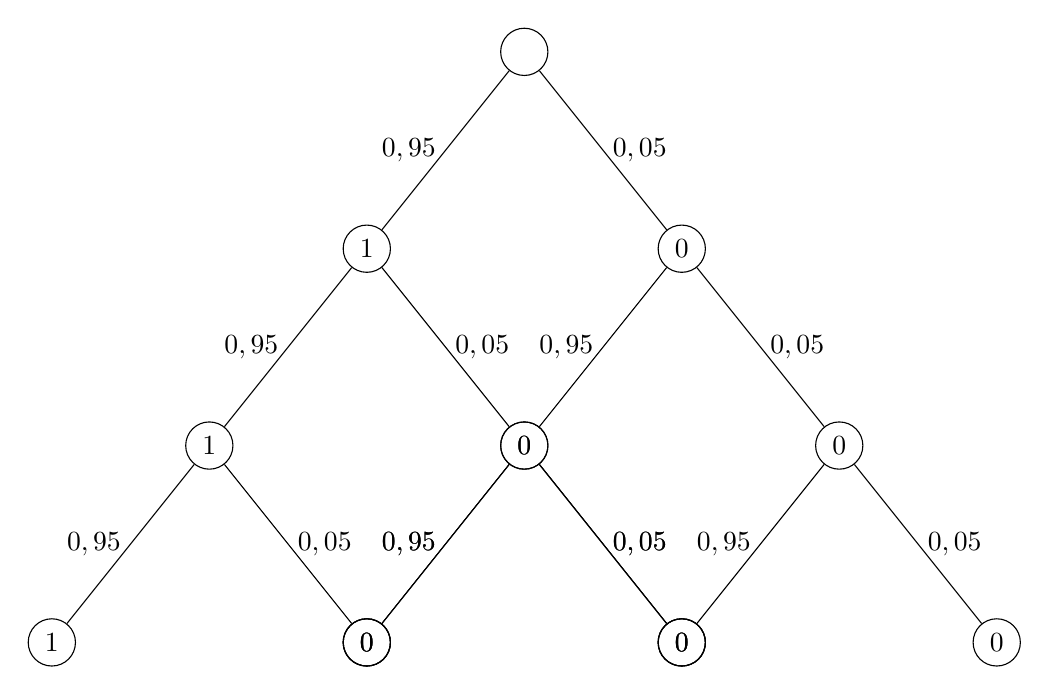
\begin{tikzpicture}[grow=down, sibling distance=4cm, level distance=2.5cm]
  \tikzset{bag/.style={circle, draw=black, minimum size=6mm, inner sep=2pt}}

  \node[bag] {}
child {
  node (A) [bag] {$1$}
  child {
    node (AB) [bag] {$1$}
    child {
      node (ABB) [bag] {$1$}
      edge from parent node[left] {$0,95$}
    }
    child {
      node (ABnB) [bag] {$0$}
      edge from parent node[right] {$0,05$}
    }
    edge from parent node[left] {$0,95$}
  }
  child {
    node (AnB) [bag] {$0$}
    child {
      node (AnBB) [bag] {$0$}
      edge from parent node[left] {$0,95$}
    }
    child {
      node (AnBnB) [bag] {$0$}
      edge from parent node[right] {$0,05$}
    }
    edge from parent node[right] {$0,05$}
  }
  edge from parent node[left] {$0,95$}
}
  child {
  node (nA) [bag] {$0$}
  child {
    node (nAB) [bag] {$0$}
    child {
      node (nABB) [bag] {$0$}
      edge from parent node[left] {$0,95$}
    }
    child {
      node (nABnB) [bag] {$0$}
      edge from parent node[right] {$0,05$}
    }
    edge from parent node[left] {$0,95$}
  }
  child {
    node (nAnB) [bag] {$0$}
    child {
      node (nAnBB) [bag] {$0$}
      edge from parent node[left] {$0,95$}
    }
    child {
      node (nAnBnB) [bag] {$0$}
      edge from parent node[right] {$0,05$}
    }
    edge from parent node[right] {$0,05$}
  }
  edge from parent node[right] {$0,05$}
};
\end{tikzpicture}}
\newline
\begin{center}
 
\renewcommand{\arraystretch}{1.3}
\setlength{\tabcolsep}{16pt}
\begin{tabular}{|c|c|c|}
\hline
\rowcolor{green!15}
$\omega$ & $P(\omega)$ & $X=x$\\
\hline
111 & $0{,}95^{3}$                 & 3\\
\hline
110 & $0{,}95^{2}\cdot 0{,}05$     & 2\\
\hline
101 & $0{,}95^{2}\cdot 0{,}05$     & 2\\
\hline
100 & $0{,}95\cdot 0{,}05^{2}$     & 1\\
\hline
011 & $0{,}95^{2}\cdot 0{,}05$     & 2\\
\hline
010 & $0{,}95\cdot 0{,}05^{2}$     & 1\\
\hline
001 & $0{,}95\cdot 0{,}05^{2}$     & 1\\
\hline
000 & $0{,}05^{3}$                 & 0\\
\hline
\end{tabular}
   
\end{center}
 \begin{bsp}{}{}
Durch das obige Baumdiagramm ist folgendes Bernoulli-Experiment simuliert. \\ In einer Urne befinden sich \(19\) weiße und eine schwarze Kugel. Aus dieser Urne werden drei Kugeln \textbf{mit zurücklegen} gezogen und  \(1\) für eine weiße Kugel bzw. \(0\) für eine schwarze notiert. Das Zufallsexperiment kann damit durch eine Bernoulli-Kette der Länge \(3\) mit dem Parameter \(p=\dfrac{19}{20} = 0,95\) beschrieben werden. Die ZG \(X\) gibt die Anzahl der weißen Kugeln an. \\[0.2cm]
Aus der obigen Tabelle ist zu sehen, dass es 3  unterschiedliche Pfade für \(2\) Treffer, also \(X=2\),  gibt. Daraus ist leicht zu berechnen, dass \(P(X=2) = 3\cdot 0,95^2\cdot 0,05\) gilt.\\[0.2cm] Verallgemeinert kann man sehen, dass für die Anzahl der Pfade \(\binom{3}{k}\) gilt und sich die passende Wahrscheinlichkeit mit\\[0.2cm]  \(P(X=k) =\binom{3}{k} \cdot 0,95^k \cdot 0,05^{3-k} \)
\end{bsp}
\begin{satz}{Wahrscheinlichkeit in einer Bernoulli-Kette}{}\index{Zufallsgröße!Binomialverteilung!Wahrscheinlichkeit}
    Gegeben ist eine Bernoulli-Kette der Länge \(n\) mit \(n \in \mathds{N}\setminus\{0\}\) und der Trefferwahrscheinlichkeit \(p\). Die Zufallsgröße \(X\) gibt die Anzahl der Treffer an. \\[0.2cm]
    Dann beträgt die Wahrscheinlichkeit für genau \(k\) Treffer mit \(k\in\{0;1;2;3;\ldots ; n\}\) \\ \(P(X=k) = \binom{n}{k}\cdot p^k \cdot \left(1-p\right)^{n-k}\)
\end{satz}
\begin{defi}{Die Binomialverteilung}{}\index{Zufallsgröße!Binomialverteilung}
 Eine Zufallsgröße \(X\) heißt binomialverteilt nach \(P^n_p(X=k) = B(n,p)\) oder \(B(n,p)\)-verteilt, wenn gilt:
 \begin{itemize}
    \item \(n\) ist die Länge der Bernoulli-Kette
    \item \(p\) ist die Trefferwahrscheinlichkeit
     \item \(X\) kann die Werte \(0;1;2;3; \ldots ; n\) mit \(n\in \mathds{N}\setminus \{0\}\) annehmen,
     \item \(P(X=k) = \binom{n}{k}\cdot p^k \cdot \left(1-p\right)^{n-k}\) mit \(0\leq p\leq 1\).
 \end{itemize}
\end{defi}
\subsection{Die kumulative Binomialverteilung}
\index{Binomialverteilung!Kumulative}\index{Zufallsgröße!Binomialverteilung!Kumulative}
Durch die Anwendung zur Berechnung der Wahrscheinlichkeiten innerhalb der Bernoulli-Kette ist es möglich, auch ohne ein Baumdiagramm die Wahrscheinlichkeit einzelner Äste zu berechnen. In vielen Aufgaben muss man allerdings sehr viele einzelne Wahrscheinlichkeiten berechnen und addiere. In diesen Fällen kann man die kumulative Binomialverteilung \(F(n;p;k)\) einer ZG \(X\) nutzen.
\begin{satz}{Die kumulative Binomialverteilung}{}
Die kumulative Verteilung \(F(n;p;k)\) einer binomialverteilten ZG \(X\) ist damit\[F(n;p;k) = F^n_p(k) = P^n_p(X\leq k) = \sum\limits_{i=0}^k \binom{n}{i} \cdot p^{i}\cdot (1-p)^{n-i}\]
\end{satz}

\subsection{Anwendung der kumulativen Verteilung}

Häufig interessiert die Wahrscheinlichkeit, dass in einer Bernoulli-Kette mindestens ein Treffer auftritt. Das ist die Summe der Wahrscheinlichkeiten für einen Treffer, zwei Treffer, drei Treffer, \(\ldots\),  n Treffer. Diese Wahrscheinlichkeit lässt sich viel einfacher durch das \textit{Gegenereignis} \textbf{kein Treffer} berechnen.
\begin{satz}{Mindestens 1 Treffer}{}\index{Binomialverteilung!Mindestens ein Treffer}
    Die Wahrscheinlichkeit mindestens ein Treffer bei einer binomialverteilten ZG \(B(n,p)\) lässt sich mit der Gegenwahrscheinlichkeit kein Treffer sehr leicht berechnen. \[P_p^n(X\geq 1) = 1- P_p^n(X=0) = 1-q^n = 1- \left(1-p\right)^n\]
\end{satz}
Häufig tauchen in diesem Zusammenhang auch Fragestellungen auf, bei denen man entweder die Trefferwahrscheinlichkeit \(p\) oder die Kettenlänge \(n\) bestimmen muss. Da in der Fragestellung dreimal das Wort mindestens auftritt, nennt man solche Aufgaben 3-m-Aufgaben. 
\begin{bem}{3-m-Aufgaben}{}\index{Binomialverteilung!3-m-Aufgaben}
\setlength{\columnsep}{10mm}
\begin{multicols}{2}
\begin{enumerate}
    \item \textbf{Mindest-Trefferwahrscheinlichkeit $p$ bei gegebenem $n$}\\
    Wie groß muss die Wahrscheinlichkeit \(p\) \textbf{mindestens} sein, damit sich unter 5 Fahrradfahrern mit einer Wahrscheinlichkeit von \textbf{mindestens} \(90\%\) \textbf{mindestens} ein Helmträger befindet?
    \begin{equation*}
        \begin{split}
            P^5_p(X\geq 1) &\geq 0,9\\
            1-P^5_p(X=0)&\geq 0,9\\
            1-(1-p)^5 &\geq 0,9 \hspace{0.3cm}|\hspace{0.1cm} -1\\
            -(1-p)^5 &\geq -0,1 \hspace{0.3cm}|\hspace{0.1cm} \cdot(-1)\\
            (1-p)^5 &\leq 0,1 \hspace{0.3cm}|\hspace{0.1cm} \sqrt[5]{\hspace{0.5cm}}\\ 
            1-p &\leq \sqrt[5]{0,1} \hspace{0.3cm}|\hspace{0.1cm} -1 \\
            -p &\leq \sqrt[5]{0,1} -1 \hspace{0.3cm}|\hspace{0.1cm} \cdot (-1)\\
            p&\geq 1-\sqrt[5]{0,1} \approx 0,3690\\ &\approx 37\%
        \end{split}
    \end{equation*}
    Die Wahrscheinlichkeit für einen Helmträger muss damit mindestens \(37\%\) betragen.
    \item \textbf{Mindest-Anzahl an Versuchen $n$ bei gegebenem $p$}\\
    Die Wahrscheinlichkeit, dass ein Radfahrer einen Helm trägt, ist \(60\%\). Wie viele Radfahrer muss man \textbf{midenstens} betrachten, damit sich darunter mit einer Wahrscheinlichkeit von \textbf{mindestens} \(99,9\%\) \textbf{mindestens} ein Helmträger befindet. 
    \begin{equation*}
        \begin{split}
            P^n_{0,6}(X\geq 1) &\geq 0,999\\
            1-P^n_{0,6}(X=0)&\geq 0,999\\
            1-(0,4)^n &\geq 0,999 \hspace{0.3cm}|\hspace{0.1cm} -1\\
            -(0,4)^n &\geq -0,001 \hspace{0.3cm}|\hspace{0.1cm} \cdot (-1)\\
            (0,4)^n &\leq 0,001\hspace{0.3cm}|\hspace{0.1cm} \ln{(\hspace{0.3cm})}\\
            n\cdot \ln{(0,4)} &\leq \ln{(0,001)}\hspace{0.3cm}|\hspace{0.1cm} : \ln{(0,4)}\\
           n&\geq \frac{\ln{(0,001)}}{\ln{(0,4)}} \approx 7,5
        \end{split}
    \end{equation*}
    Es müssen mindestens 8 Radfahrer untersucht werden.
\end{enumerate}
\end{multicols}
\end{bem}
\subsection{Typische Formulierungen}
\begin{bem}{Typische Formulierungen}{}
    \begin{center}
    
\begin{tabular}{p{0.94\linewidth}}
\hline
\textbf{Typische Aufgabenformulierungen bei }$X\sim\mathrm{Bin}(n,p)$\\[6pt]

\textbf{Der Rechner liefert:}\qquad \(\mathrm{Binomial\;CD}(x;N,p)=P^n_p(X\le x)\)\\[6pt]

\textbf{So übersetzt du Texte in Casio-Eingaben:}\\[4pt]
\(\boxed{P^n_p(X\le x)}\) \quad „\textbf{höchstens} \(x\) Treffer“ \quad\(\Rightarrow\)\quad direkt \(\mathrm{CD}(x)\)\\[4pt]

\(\boxed{P^n_p(X< x)}\) \quad „\textbf{weniger als} \(x\) Treffer“ \quad\(\Rightarrow\)\quad \(\mathrm{CD}(x-1)\)\\[4pt]

\(\boxed{P^n_p(X\ge x)}\) \quad „\textbf{mindestens} \(x\) Treffer“ \quad\(\Rightarrow\)\quad \(1-\mathrm{CD}(x-1)\)\\[4pt]

\(\boxed{P^n_p(X> x)}\) \quad „\textbf{mehr als} \(x\) Treffer“ \quad\(\Rightarrow\)\quad \(1-\mathrm{CD}(x)\)\\[6pt]

\textbf{Entsprechend bei „nicht mehr als / nicht weniger als“:}\\[4pt]
„\textbf{nicht mehr als} \(x\)“ \(\Leftrightarrow P^n_p(X\le x)\) \(\Rightarrow\) \(\mathrm{CD}(x)\)\\[4pt]
„\textbf{nicht weniger als} \(x\)“ \(\Leftrightarrow P^n_p(X\ge x)\) \(\Rightarrow\) \(1-\mathrm{CD}(x-1)\)\\[6pt]

\textbf{Zwischen zwei Werten:}\\[4pt]
\(\boxed{P^n_p(a\le X\le b) = P^n_p(X\leq b) - P^n_p(X\leq a-1)} \) \quad\(\Rightarrow\)\quad \(\mathrm{CD}(b)-\mathrm{CD}(a-1)\)\\[4pt]
\(\boxed{P^n_p(a< X\le b)= P^n_p(X\leq b) - P^n_p(X\leq a)}\) \quad\(\Rightarrow\)\quad \(\mathrm{CD}(b)-\mathrm{CD}(a)\)\\
\hline
\end{tabular}
\end{center}

\end{bem}
\subsection{Taschenrechner Anleitungen}\index{Zufallsgröße!Binomialverteilung!Taschenrechner}
\begin{b8d}{Berechnung der kumulativen Binomialverteilung}{}
\begin{center}
\begin{tabular}{p{0.94\linewidth}}
\hline
\textbf{Route zur Binomial CD-Funktion}\\[4pt]
1) \taste{MODE/SETUP} \;\(\rightarrow\)\; Auswahlmenü\\
2) \taste{4} \;\(\rightarrow\)\; \textbf{DIST} (Verteilung)\\
3) Mit dem Cursor auf \textbf{Seite 2} wechseln \;\(\rightarrow\)\; \textbf{Binomial CD}\\
4) \taste{2} \;\(\rightarrow\)\; \textbf{Variablen eingeben}\\[4pt]
\textbf{Eingabereihenfolge:}\\
Zuerst \(\;x\) (Wert der Zufallsgröße) \(\rightarrow\) dann \(\;N\) (Kettenlänge) \(\rightarrow\) dann \(\;p\) (Trefferwahrscheinlichkeit).\\
\hline
\end{tabular}
\end{center}
\noindent
\textbf{Was rechnet Binomial CD hier?} In diesem Modus liefert der Rechner typischerweise
\[
\boxed{\text{Binomial CD}(x;N,p)=P^n_p(X\le x)}
\]
Also: „höchstens \(x\) Treffer“.
\end{b8d}
\begin{b8d}{Berechnung der Wahrscheinlichkeit in den Taschenrechner}{}
\begin{center}
\begin{tabular}{p{0.94\linewidth}}
\hline
\textbf{Route zur Funktion für exakt \(k\) Treffer (Binomial PD)}\\[4pt]
1) \taste{MODE/SETUP} \;\(\rightarrow\)\; Auswahlmenü\\
2) \taste{4} \;\(\rightarrow\)\; \textbf{DIST} (Verteilung)\\
3) \taste{4} \;\(\rightarrow\)\; \textbf{Binomial PD} (Probability Distribution)\\
4) \taste{2} \;\(\rightarrow\)\; \textbf{VAR} (Variablen eingeben)\\[6pt]
\textbf{Eingabereihenfolge:}\\
Zuerst \(\;x\) (Wert der Zufallsgröße) \(\rightarrow\) dann \(\;N\) (Kettenlänge) \(\rightarrow\) dann \(\;p\) (Trefferwahrscheinlichkeit).\\
\hline
\end{tabular}
\end{center}

\noindent
\textbf{Was rechnet Binomial PD?}
\[
\boxed{\text{Binomial PD}(x;N,p)=P^n_p(X=x)}
\]
Also: „genau \(x\) Treffer“.
\end{b8d}
\begin{b8d}{Berechnung der Binomialverteilung als Tabelle}{}
\begin{center}
\begin{tabular}{p{0.94\linewidth}}
\hline
\textbf{Route zur Binomialverteilung als Tabelle (LIST)}\\[4pt]
1) \taste{MODE/SETUP} \;\(\rightarrow\)\; Auswahlmenü\\
2) \taste{4} \;\(\rightarrow\)\; \textbf{DIST} (Verteilung)\\
3) \taste{3} \;\(\rightarrow\)\; \textbf{Binomial PD} \quad(\textit{Einzelwahrscheinlichkeiten})\\
4) \taste{1} \;\(\rightarrow\)\; \textbf{LIST} \quad(\textit{Tabelleneingabe})\\[6pt]

\textbf{Eingabereihenfolge:}\\
Zuerst die gewünschten \(x\)-Werte in der Liste (z.\,B. \(0,1,2,\dots\)) \(\rightarrow\)
dann \(\;N\) (Kettenlänge/Anzahl der Versuche) \(\rightarrow\)
dann \(\;p\) (Trefferwahrscheinlichkeit).\\[4pt]

\textbf{Ausgabe:}\\
In der Ergebnisspalte erscheint zu jedem eingetragenen \(x\) der Wert
\(\;P^n_p(X=x)\).\\
\hline
\end{tabular}
\end{center}

\noindent
\textbf{Was liefert die Tabelle hier?} In diesem Modus berechnet der Rechner
\[
\boxed{\mathrm{Binomial\;PD}(x;N,p)=P^n_p(X=x)}
\]
also: „genau \(x\) Treffer“ (für jedes \(x\) aus der Liste).
\end{b8d}
\begin{b8d}{Berechnung der kumulativen Binomialverteilung als Tabelle}{}
\begin{center}
\begin{tabular}{p{0.94\linewidth}}
\hline
\textbf{Route zur kumulativen Binomialverteilung als Tabelle (LIST)}\\[4pt]
1) \taste{MODE/SETUP} \;\(\rightarrow\)\; Auswahlmenü\\
2) \taste{4} \;\(\rightarrow\)\; \textbf{DIST} (Verteilung)\\
3) Mit dem Cursor auf \textbf{Seite 2} wechseln \;\(\rightarrow\)\; \textbf{Binomial CD}\\
4) \taste{1} \;\(\rightarrow\)\; \textbf{LIST} \quad(\textit{Tabelleneingabe})\\[6pt]

\textbf{Eingabereihenfolge:}\\
Zuerst die gewünschten \(x\)-Werte in der Liste (z.\,B. \(0,1,2,\dots\)) \(\rightarrow\)
dann \(\;N\) (Kettenlänge/Anzahl der Versuche) \(\rightarrow\)
dann \(\;p\) (Trefferwahrscheinlichkeit).\\[4pt]

\textbf{Ausgabe:}\\
In der Ergebnisspalte erscheint zu jedem eingetragenen \(x\) der Wert
\(\;P^n_p(X\le x)\).\\
\hline
\end{tabular}
\end{center}

\noindent
\textbf{Was liefert die Tabelle hier?} In diesem Modus berechnet der Rechner
\[
\boxed{\mathrm{Binomial\;CD}(x;N,p)=P^n_p(X\le x)}
\]
also: „höchstens \(x\) Treffer“ (für jedes \(x\) aus der Liste).
\end{b8d} 

\section{Hypothesentest}\index{Hypothesentest}
\begin{itemize}
\item Zwei sich ausschließende Hypothesen werden betrachtet
\begin{enumerate}
\item Nullhypothese $H_0$ 
\item Gegenhypothese $H_1$
\end{enumerate}
\item Anzahl der Treffer einer \textcolor{red}{Stichprobe} mit festgelegter Länge bildet die \textcolor{red}{Testgröße}
\item Wertebereich der Testgröße wird in den \textcolor{red}{kritischen Bereich} K (\textcolor{red}{Ablehnungsbereich}) und den \textcolor{red}{nichtkritischen Bereich} $\bar{K}$  (\textcolor{red}{Annahmebereich}) zerlegt
\item liegt der durch die Stichprobe gewonnene Wert der Testgröße in K, dann wird $H_0$ verworfen, ansonsten wird $H_0$ nicht verworfen (\textcolor{red}{Entscheidungsregel}). 
\item Fehler beim Testen von Hypothesen\\

\scalebox{1.2}{\begin{tabular}{|>{\columncolor{gray!15}}l|>{\columncolor{gray!10}}c|>{\columncolor{gray!10}}c|}
  \hline
  \rowcolor{gray!20}
  \textbf{Entscheidung} & \textbf{$H_0$ ist wahr.} & \textbf{$H_0$ ist falsch.} \\
  \hline
  $H_0$ wird abgelehnt. &
  \cellcolor{red!30}Fehler erster Art &
  \cellcolor{green!20}Richtige Entscheidung \\
  \hline
  $H_0$ wird nicht abgelehnt. &
  \cellcolor{green!20}Richtige Entscheidung &
  \cellcolor{cyan!20}Fehler zweiter Art \\
  \hline
\end{tabular}}
\begin{enumerate}
\item Fehler erster Art: $H_0$ wird verworfen, obwohl sie wahr ist. \index{Hypothesentest!Fehler 1. Art}
\item Fehler zweiter Art: $H_0$ wird beibehalten, obwohl sie falsch ist.\index{Hypothesentest!Fehler 2. Art}
\item Durch eine Veränderung der Entscheidungsregel kann man nur die Wahrscheinlichkeit
des Fehlers der einen Art auf Kosten der Wahrscheinlichkeit des Fehlers der anderen Art verringern.
\item Durch eine Erhöhung des Stichprobenumfangs können bei einem Test die Fehler
1. und 2. Art verringert werden. Allerdings ist eine solche Erhöhung in der Praxis auch mit erhöhten Kosten verbunden.
\end{enumerate}
\end{itemize}